\chapter{Methoden zur Abschätzung der maximalen Versorgungslänge}


%-------------------------------------

\section{Modelle}
\label{sec:2methoden}

In diesem Kapitel wird auf die Modelle und Methoden eingegangen, die bei einem\\Modellierungsvorgang durchlaufen werden. 

%============================
\subsection{Gesamtmodell-Input Netzwerkgraph}
\label{sec:2 modelle}

\vspace{0.5cm}
Die Ausführungen zum Thema Gesamtmodell, welche in diesem Kapitel behandelt werden, beziehen sich auf \cite{pinkafeld1}, sofern nicht anders angegeben.
\\ 
\par Ein Anschlussbereich wird wie folgt als Netzwerkgraph dargestellt. $G=(V,E)$ mit $V$ als Menge von Knoten und $E$ als Menge der Kanten. 
Die Erstellung von Knoten und Kanten wird unter der Berücksichtigung der Geodaten-Attribute aus Kapitel 2.2.1 realisiert.

\vspace{0.3cm}
Jeder Knoten $v\in V$ besitzt die folgenden Attribute: 



\begin{itemize}
\item geographische Position $x-Koordinate, y-Koordinate ~in~ der~ digitalen~Katastralmappe ~$
\item Informationsbedarf $\pi(v) \in \mathds{N}_{(0)},v \in V~$
\end{itemize}


Der Informationsbedarf wird auf Basis der Mikrozellendaten identifiziert. Besitzt ein Knoten keinen Informationsbedarf, dann wird er mit $~\pi(v)=0~$belegt.
Man spricht von einem spatialen Knoten, welcher nur aufgrund der Graphen-Konstruierung in der digitalen Katastralmappe (DKM) enstanden ist.\\
Besitzt ein Knoten einen Informationsgehalt, gilt die Forderung $\pi(v)>0$, es handelt sich um ein Anschlussobjekt.
Es gilt zu beachten, ob das Anschlussobjekt mit Kupferkabeln oder aber mit Glasfaserkabeln versorgt wird. Wird das Anschlussobjekt mit Kupferkabeln in
das Netzwerk integriert, dann gibt der Informationsbedarf die Anzahl der Teilnehmeranschlusseinrichtungen wie zum Beispiel von Telefonen an. 
Diese Teilnehmer werden mit kurzen Stichleitungen, sogenannten \textit{drop-wires} versorgt. 
Wird der Teilnehmer mit Lichtwellenleitern angebunden, so gibt der Informationsbedarf die Anzahl der Wellenlängen wieder, für welche eine entsprechende
Anzahl von \textit{drop-wires} gedemultiplexed werden müssen. 
Kanten $e \in E$ können auch Verbindungstrassen von spatialen Knoten und Anschlussobjekten sein. 


%---------------------------------------------
\subsubsection{Workflow}
\label{sec:2 modelle}


\vspace{0.5cm}

\par Nachfolgend wird der Workflow eines Modelldurchlaufes beschrieben. Dieser wird grundsätzlich in zwei Schritten ausgeführt.
Im ersten Schritt wird ein Top-down Clustering durchgeführt, auf welches eine Bottom-up Optimierung folgt.
Um einen Modelldurchlauf zu ermöglichen, müssen die Inputdaten erstellt werden. Dies wird im nachfolgenden Kapitel 2.1.2 erläutert. 
%---------------------------------------------
\vspace{1cm}

\subsection{Normierte Geodaten}
\label{sec:2 modelle}


\vspace{0.5cm}

{\em Normierte Geodaten stellen die generalisierten, topologisch korrekten Nutzungsflächen der\\ digitalen Katastralmappe (DKM) dar, die um für die
Graphgenerierung relevante Flächen wie Straßenkreuzungsflächen und Querungsflächen (Eisenbahnübergänge, Brücken über Gewässer) automatisiert
bzw. semiautomatisiert erweitert werden}\cite{prossegger1}.

\ Aufgrund von räumlichen Analysen und auf Vertriebsinformationen basierend, werden branchenspezifische Umsatzpotentiale für Standorte der
Anschlussobjekte bestimmt. Hierbei werden die Faktoren der bestehenden Netzinfrastruktur und die nutzbare Infrastruktur in den 
Geobasisdatensatz integriert. Als bestehende Netzwerkinfrastruktur versteht sich das Strom- und Glasfasernetz, und unter nutzbarer Infrastruktur
werden unter anderem existierende Leerverrohrungen, welche es zu nutzen gilt, verstanden. Die Umsetzung erfolgt mittles eines FME (Feature Manipulation
Engine)-Modells, in welchem eine automatisierte Aufbereitung des jeweiligen Gebietes auf Basis der definierten Geobasisdaten erfolgt\cite{prossegger1}.

\begin{figure}[H]
    \centerline{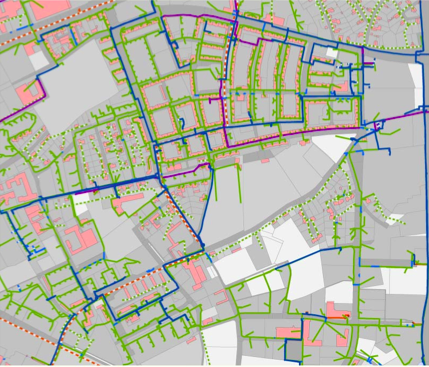
\includegraphics[scale=0.5]{pics/dkm.png}}
    \caption[Digitale Katastralmappe]{\label{FiG:Digitale Katastralmappe }
	Ausschnitt der digitalen Katastralmappe\cite{prossegger1}}
\end{figure}



%---------------------------------------------
\subsubsection{Top-Down Clustering}
\label{sec:2methoden}


\vspace{0.5cm}

Um Netzwerke zu optimieren ist es sinnvoll diese in Hierarchien einzuteilen. Eine Unterteilung in ein hierarchisches Netzwerk wird in Folge beschrieben. 
Dafür wird der Netzwerkgraph $G$ in Teilgraphen $H_{i}\subset G,
~i=1,...,m$ zerteilt. Jeder dieser entstandenen Teilgraphen spiegelt nun einen Accessnetzbereich (eine Ebene tiefer) wieder. Weiters wird jeder entstandene
Teilgraph $H_{i}$ weiter zerteilt in $K_{i,j}\subset H_{i}, ~j=1,...,n_{i}$ und es ergibt sich nun das Accesszellennetz. Man erhält $K_{i,j}$ für die
$j$-te Accesszelle im $i$-ten Accessnetz vom Teilgraphen $H_{i}$. 
\par Somit wurde ein Netzwerkgraph in eine Drei-Ebenen-Hierarchie unterteilt.
Dieser Vorgang wird als Top-Down Clustering des Anschlussbereiches $G$ bezeichnet.
\vspace{0.5cm}

In diesem Abschnitt der Modellierung wird die Implementierung eingebettet. Es wird ein zusätzlicher Parameter eingeführt, welcher die Begrenzung der 
maximalen Anschlusslänge reguliert. So kann der Input des Routing-Modells kontrolliert beziehungsweise reguliert werden.


%---------------------------------------------


\subsubsection{Bottom-up Optimierung}
\label{sec:2methoden}


\vspace{0.3cm}

Um eine Simulation bezüglich der Kosten optimieren zu können, wird das Netzwerk vom Grund auf neu, also Bottom-up simuliert.
Die Teilgraphen $T'$ stellen kostenoptimierte, mit dafür entsprechenden Modellen berechnete, Netzwerktrassierungen dar.

%-----------------------------------------------

\vspace{1cm}
\subsection{Cluster-Modell}
\label{sec:2 modelle}


\vspace{0.5cm}

\par Wählamtsbereiche, die als Ausgangspunkt dieser Berechnung dienen, werden durch Zerlegung des Ausgangsgraphen in Beziehung zur den vorhin definierten
Ebenen (Kapitel 1.3) unterteilt. 
Mit Hilfe einer Toolbox, welche im bestehenden Programm implementiert ist, werden Wählamtsbereiche in kleinere Subgebiete, den Accessnetzen, unterteilt. 
Die sich ergebenden Accessnetzebenen werden abermals unterteilt, wobei man als Output die Accesszellebenen erhält. Der gesamte Vorgang der Zerlegung eines
Gebietes in kleinere Subgebiete wird als Clustern bezeichnet und verläuft in einer Top Down Strategie.

\par Hierbei wird für einen Netzwerkgraphen $G=(V,E)$ eine Zerlegung in Teilgraphen\\ vorgenommen. Teilgraphen werden als $G' =(V,E)$ bezeichnet.
Durch die Dilatation eingeschränkt, wird diese Graphenzerlegung durchgeführt. 
\vspace{0.3cm}

\par Die Dilatation wird formal wie folgt beschrieben: 
\\
\begin{equation}
\sum_{i=1}^{m}  max \left\lbrace\| u-v \|_{2} ~:u,v \in V_{i} \times V_{i} ~ mit ~\pi(u) >0,\pi(v) >0\right\rbrace
\end{equation} 
\\
Es gilt die Teilgraphanzahl $m$und den minimalen Teilgraphdurchmesser zu finden,  wobei die maximale Versorgungslänge auf den Teilgraphdurchmesser beschränkt ist.
\\
\begin{equation} 
~max~\left\lbrace\| u-v \|_{2}~:u,v \in V_{i} \times V_{i} ~ und~\pi(u)>0,\pi(v)>0\right\rbrace\leq ~ d_{max} ~f\ddot{u}r~ i=1,...,m  
\end{equation} 
\\
Weiters gilt es, die Bedingung des Gesamtinformationsbedarfs zu berücksichtigen. Die Summen der Teilinformationsbedürfnisse aller Teilgraphen dürfen den Gesamtinformationsbedarf nicht überschreiten.
\\
\begin{equation}
\sum_{v\in V_{i}} \pi(v) \leq \pi_{max}  ~f\ddot{u}r~  i=1,...,m ~   
\end{equation} 
\\
\begin{figure}[H]
    \centerline{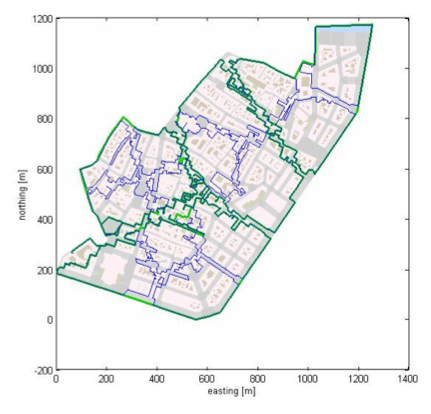
\includegraphics[scale=0.5]{pics/Cluster_Abbildung.png}}
    \caption[Bereichsunterteilung in Cluster]{\label{FiG:Bereichsunterteilung in Cluster } 
	Bereichsunterteilung nach dem Cluster-Modell, ersichtlich ist die Einteilung in Accessnetze (grün) und Accesszellen (blau)\cite{tech_rep_1} }
\end{figure}

Es gibt zwei unterschiedliche Möglichkeiten das Clustern durchzuführen:


\begin{itemize}
\item Barrier Clustering
\item Dens Clustering
\end{itemize}


\par Wird die Forderung (2.1 Dilatation) dadurch ersetzt, dass alle Kanten, welche die Teilgraphen $H_{i}$
miteinander verbinden, zu einer oder auch mehreren Nutzungsklassen gehören müssen, so wird vom Barrier-Clustering Model gesprochen.
Für dieses Modell ist die Lösung heuristisch. Beim Verwenden von Barrier-Clustering werden die Teilgraphen durch
Breitensuche solange initialisiert, bis man auf Kanten mit vorgegebenen Nutzungen stößt.

\vspace{0.5cm}
\par  Verwendet man Dens-Clustering, kann für ein gegebenes $m$ eine exakte Lösung gefunden werden.  
Wird die Lösung von den Forderungen 2.2 oder 2.3 verletzt,  dann wird $m$ solange erhöht, bis sie wieder erfüllt sind.
Im Anschluss werden die Teilgraphen vereinigt, bis eine der Bedingungen, 2.2 oder 2.3, verletzt wird.


\vspace{1cm}

% --------------------------------------------------------------------------

\subsection{Routing-Modell}
\label{sec:2 modelle}


\vspace{0.5cm}

\par Nach dem Clustern der unterschiedlichen Ebenen in Citynetz, Accessnetz  und Accesszellen ist es nun möglich Trassen in den einzelnen Teilbereichen zu
berechnen. Beeinflussend auf die Wahl der Trassierung wirken Faktoren wie zum Beispiel Kosten für Trassenführung. Diese Kosten setzen sich aus mehreren
Faktoren, wie zum Beispiel unter anderem den Widmungsklassen, zusammen. 
\\
Ergo ist es günstiger eine Verlegetrasse durch ein unbebautes Gebiet zu erstellen, während im
innerstädtischen Bereich die Kosten dafür wesentlich höher sind.
Diese sind in den Bereichen ländlich und innerstädtisch signifikant unterschiedlich und wirken nun auf die Erstellung eines Trassenverlaufes ein.\\ Besondere
Rücksicht wird unter anderem auf Gewässer genommen. 
Die Kosten, um diese zu durchqueren, sind im Vergleich zu einer Trassenführung auf festem Boden,
wesentlich höher.
Um dem entgegenzusteuern wird dieser Parameter per default hoch angesetzt. 
Aufgrund dessen kann es vorkommen, dass es einzelne Anschlussobjekte gibt, welche über einen überdurchschnittlich langen Weg angebunden werden müssen
\cite{tech_rep_1}.

 \vspace{0.5cm}
 
\par Um solche Anschlusslängen zu vermeiden, werden die Versorgungslängen bereits im Cluster-Modell berücksichtigt. Somit können sich im Routing-Modell
solch lange Trassenführungen nicht mehr ergeben, da das Längenmaximum bereits zuvor festgelegt wurde. Die Anschlussobjekte müssen nun einem anderen 
Cluster zugeteilt werden, um eine Optimierung bezüglich der Längenbegrenzung zu gewährleisten.\\
Nachdem die Routen für alle Teilbereiche (Bottom Up) kostenoptimiert, bezüglich der Trassierungslänge, erstellt wurden, sind die
Routinginformationen in vorgefertigten Dateien aufbereitet.\\
Das Routing-Modell berechnet die Trassierung auf Basis des gegebenen Graphen. Dieser Graph wird vom Cluster-Modell aufbereitet und bereitgestellt. 
Es ist nun möglich eine kostenoptimierte Trassierung in den einzelnen Subgebieten eines Wählamtsbereichs zu simulieren. 
Dabei wird eine Bottom Up – Strategie verfolgt. Das bedeutet, dass zuerst alle Accesszellen, anschließend alle Access- und danach Citynetze 
geroutet werden.
In jeder dieser Hierarchien werden die Kanten so ausgewählt, dass in jedem Anschlussbereich

\begin{enumerate}
		\item[a.] genau eine Verbindung zwischen jedem enthaltenen Anschlussobjekt und einem Versorgungszentrum oder 
		\item[b.] zwei knotendisjunkte Verbindungen für jedes Paar von Anschlussobjekten zum Versorgungszentrum existiert
\end{enumerate}

und die Summe der Kosten der gewählten Kanten ein Minimum ist.		



 
\vspace{1cm}
% --------------------------------------------------------------------------

\section{Mathematisches Konzept}
\label{sec:2methoden}


\vspace{0.5cm}

Für nachfolgendes Kapitel ist es notwendig einige Begriffe vorab zu erklären.

\subsection{Baum}
\label{sec:2methoden}

\vspace{0.5cm}

Ungerichtete Graphen können in Form eines Baumes dargestellt werden.
\vspace{0.3cm}

Ein ungerichteter Graph $G$ ist dann ein Baum, wenn:

\begin{enumerate}
\item $G$ ist zusammenhängend und $m=n-1$;
\item$G$ enthält keinen geschlossenen Weg und $m=n-1$;
\item In $G$ gibt es zwischen jedem Paar genau einen Weg;
\end{enumerate}

\vspace{0.3cm}

\begin{graybox}
\textbf{\textit{Definition:}} Ein ungerichteter Graph $G=(V, E, \gamma)$ heißt Wald, wenn $G$ kreisfrei ist, also keinen elementaren Kreis besitzt. Falls$~G~$ zusätzlich zusammenhängend ist, so heißt $G$ Baum\cite{krumke1}.
\end{graybox}

\vspace{1cm}

\begin{flushleft}
Desweiteren besteht ein Baum aus folgenden Elementen:
\end{flushleft}


\begin{itemize}
\item Kanten
\item Knoten
\end{itemize}

Knoten sind über Kanten miteinander verbunden. Wurzel und Blätter sind Sonderformen von Knoten. Die Wurzel ist der Startpunkt eines Graphen. 
Blätter hingegen sind die Enden eines Baumes, zu ihnen führt nur eine Kante. 

\vspace{1cm}
\subsection{Steiner Baum}
\label{sec:2methoden}


\vspace{0.5cm}

Ist $G=(V, E )$ ein vollständiger Graph mit Kantengewichten $c: E \to \mathbb{R}_{+}$, so scheint bei flüchtiger Betrachtung das Problem, einen
gewichtsminimalen Steiner Baum für die Terminalmenge $K$ zu finden, identisch damit zu sein, einen minimalen spannenden Baum im (vollständigen) 
induzierten Subgraphen $G[K]$ zu bestimmen. Eine nähere Betrachtung zeigt aber, dass ein minimaler spannender Baum in $G[K]$ nicht zwangsweise ein minimaler Steiner Baum ist.
\\


\vspace{0.5cm}

\begin{graybox}
\textbf{\textit{Definition:}} Sei $G=(V, E )$ ein ungerichteter Graph und $K \subseteq V$ eine beliebige Teilmenge der Eckenmenge. Ein Steinerbaum
 in $G$ für die Menge$K$ ist ein Teilgraph $T \sqsubseteq G$, der ein Baum ist und dessen Eckenmenge $K$ umfasst: $K \subseteq V(T)$.
Die Elemente von $~K~$ nennt man Terminale, die Ecken aus $V(T) \setminus K~ Steinerpunkte$\cite{krumke1}.
\end{graybox}

\vspace{1cm}


\subsection{Vorabschätzung über MST Ansatz}
\label{sec:2methoden}


\vspace{0.5cm}

Derzeit wird ein Steiner Baum zum Bestimmen der Trassierung verwendet. Mittels MST soll nun eine Abschätzung noch vor dem Routing-Modell 
durchgeführt werden. \\
Unter einem MST versteht sich ein minimal spannender Baum eines Graphen. \\ 

\begin{graybox}
\textbf{\textit{Definition:}} Sei $G=(V, E, \gamma)$ ein ungerichteter Graph. Ein Partialgraph $H=(V,E', \gamma)$ von $G$ ist ein spannender Baum, 
wenn $H$ ein Baum ist. \\
Jeder spannende Baum von $G$ enhält mindestens $|V(G)| -1$ Kanten\cite{krumke1}.
\end{graybox}

\vspace{0.5cm}

Jeder Graph besitzt auch ein Gewicht. Das Gewicht setzt sich aus der Summe der
Kantengewichte zusammen.  Alle Knoten des Hauptgraphen müssen auch im MST enthalten sein (Abbildung 2.3). 
Ein Baum heißt minimal spannend, wenn kein anderer Spannbaum im selben Graphen, mit einem geringeren Gewicht existiert\cite{krumke1}.

\begin{figure}[H]
    \centerline{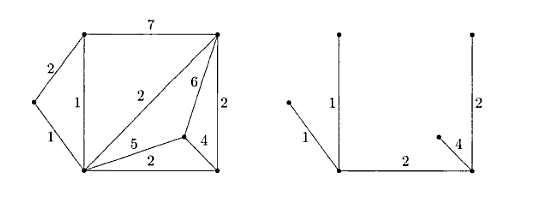
\includegraphics[scale=0.5]{pics/minimal_spannender_baum}}
    \caption[Minimal Spannender Baum-MST]{\label{FiG:Minimal Spannender Baum }
	Hauptgraph\cite{krumke1} und der Minimal Spannende Baum zu diesem \cite{krumke1}}
\end{figure}	

\par Mittels des Prim-Algorithmus wird ein minimal spannender Baum erstellt. 
Als Output\\ergibt sich ein Untergraph  $G'(V',E')$, mit den günstigsten Kanten und Knoten, welche benötigt werden, um den minimal spannenden Baum für den 
ursprünglichen Graphen $G(V,E)$ bestimmen zu können\cite{krumke1}.

\vspace{1cm}

\subsection{Leaf Backward Algorithmus}
\label{sec2:methoden}


\vspace{0.5cm}

Der Output aus Kapitel 2.2.2 stellt nun einen minimal spannenden Baum (MST) dar.\\ Spannende Bäume existieren nur in zusammenhängenden ungerichteten
Graphen.\\
In diesem MST sind noch Knoten enthalten, welche keinen Informationsbedarf
beinhalten und auch nicht als Verbindungsknoten dienen.

\vspace{0.3cm}

Nun müssen diese Bedingungen zutreffen um solche Knoten zu entfernen:

\begin{enumerate}
	\item ist der Informationsgehalt $\pi(v) = 0 $	
	\item hat der Knoten nur einen Nachbarknoten, handelt es sich um ein Blatt
\end{enumerate}

 
Es gilt für $v\in V$ folgende Bedingungen zu berücksichtigen:


\begin{enumerate}
  \item \textit{$v$ hat mehr als einen Nachbarn} 
  \item \textit{$v$ ist $\pi(v)>0$ , also ein Anschlussobjekt} \label{l2}
  \item \textit{$v$ ist als Distribution Center gekennzeichnet} \label{l3}
\end{enumerate}

Verletzt ein Knoten im Graphen eine oder mehrere dieser Bedingungen, so wird er und die zuführende Kante aus dem Graphen entfernt. 


Der Output-Graph entspricht nun einem Steiner Baum.


%==================
\subsection{Implementierungskonzept}
\label{sec:2methoden}


\vspace{0.5cm}

Die Implementierung setzt sich aus den folgenden Teilschritten zusammen. 

\begin{itemize}
  
  \item Berechnen der günstigsten Wege im Graphen - MST Algorithmus
  \item Reduzieren der redundanten Knoten mittels Leaf Backward Algorithmus 
   \item Berechnen des Flächenschwerpunktes und bestimmen des Distribution Centers
    \item Vergleich von Output Steiner Baum und MST
\end{itemize}

\begin{figure}[H]
    \centerline{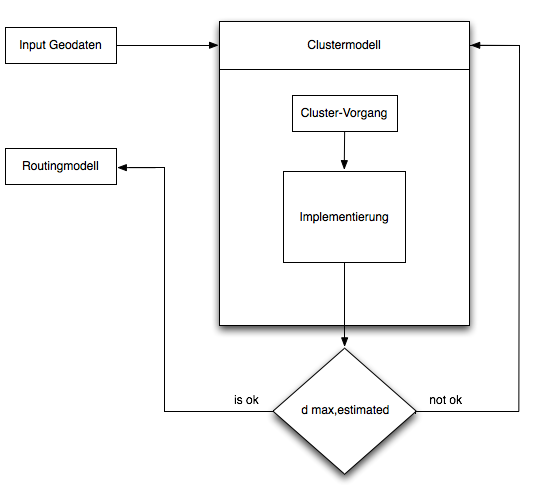
\includegraphics[scale=0.5]{pics/diagramm_1}}
    \caption[Ablaufdiagramm für Einbindung in bestehendes Programm]{\label{FiG:Ablaufdiagramm für Einbindung in bestehendes Programm }
	Ablaufdiagramm für Einbindung in bestehendes Programm}
\end{figure}

\vspace{0.5cm}

%============
\subsection{Implementierung}
\label{sec:2methoden}

\vspace{0.5cm}

Da die Einbindung in das Programm RTR\_R2008a nicht Teil dieser Arbeit ist, wird der Vorgang abgeändert durchgeführt. 
Es wird ein Testbed erstellt, in welchem die Resultate des MST-Ansatzes mit den Ergebnissen des Steiner Baumes verglichen werden.
Wie im Ablaufdiagramm (Abbildung 2.5) ersichtlich, werden nun die Schritte in Pseudo-Codes beschrieben. Da das Cluster-Modell und die Aufbereitung der
Geodaten bereits implementiert sind, werden diese im ersten Schritt nicht weiter beachtet. Somit wird mit der Berechnung des MST begonnen. Als Input 
dient hierfür ein $.ist$ File, in welchem sich die Geodaten befinden. 

\begin{figure}[H]
    \centerline{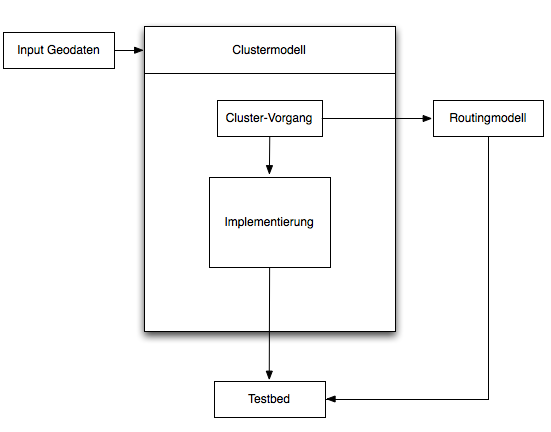
\includegraphics[scale=0.5]{pics/diagrammRealisierung}}
    \caption[Ablaufdiagramm der Realisierung]{\label{FiG:Ablaufdiagramm der Realisierung} Ablaufdiagramm der Realisierung}
\end{figure}

       
\begin{figure}[H]
    \centerline{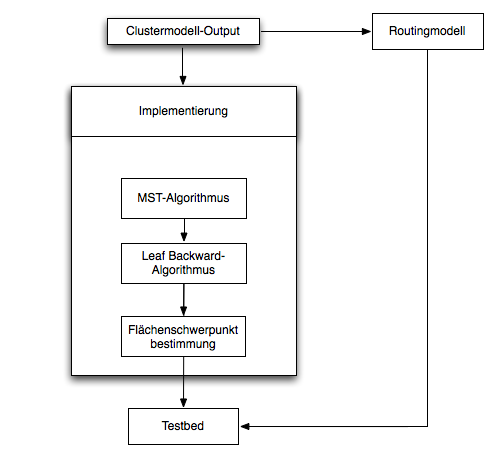
\includegraphics[scale=0.7]{pics/diagrammRealisierungDetail}}
    \caption[Ablaufdiagramm-Detail der Realisierung]{\label{FiG:Ablaufdiagramm-Detail der Realisierung} Detailansicht der realisierten Implementierung}
\end{figure}
       
       
\subsubsection{MST Algorithmus}
\label{sec:2methoden}

\vspace{0.5cm}

Um einen minimal spannenden Baum zu erhalten gibt es mehrere Möglichkeiten.  In dieser Arbeit wird der Algorithmus von Prim verwendet, 
um einen MST zu erhalten.
In diesem Algorithmus bilden die ausgewählten Kanten zu jedem Zeitpunkt einen Baum  $G=(V,E)$. Zu Beginn wird ein 
beliebiger Knoten $v \in V$ gewählt. Durch weiteres Hinzufügen der günstigsten Kanten, entsteht der gesuchte Baum\cite{turau1}. 
\vspace{0.3cm}
\par Die Auswahl der Kanten wird dabei wie folgt getroffen:

\begin{enumerate}
 \item Sei $V$ die Menge der Ecken des gesuchten Baumes $G$ und $E$ die Menge der Ecken des Graphen.
 \item Man wähle unter den Kanten $(u,v)$, deren Anfangsecke $u \in V$ und deren Endecke $v \in E \setminus V$ liegen, diejenige mit der kleinsten
 Bewertung aus. 
\item Diese wird dann in $G$ eingefügt.
\item Weiters wird $v$ in $V$ eingefügt.
\item Dieser Schritt wird solange wiederholt bis $V=E$ ist.
 \end{enumerate}


Beim Algorithmus von Prim wird das Sortieren der Kanten vermieden, jedoch ist der Aufwand der Kanten aufwändiger. Die Auswahl und Verwaltung
der Menge $V$ kann mit Hilfe eines Feldes erfolgen. Im Feld wird für jede Ecke $e \in E\setminus V$ die kleinste Bewertung unter den Kanten $(e,v)$ mit 
$v \in V$ gespeichert. Es wird auch die Endecke dieser Kante abgespeichert.
Wurde eine Kante $(e,v)$ ausgewählt wird die Ecke $e$ als zugehörig 
von $V$ markiert.
Die Laufzeit der Prim-Prozedur beträgt $n-1$ Iterationen, da bei jedem Durchlauf genau eine Ecke eingefügt wird. Der Aufwand für die 
Auswahl der Kante und das Aktualisieren des Feldes beträgt $O(n)$. Das bedeutet, der Gesamtaufwand beträgt $O(n^2)$.
Der Primalgorithmus sollte Verwendung finden, wenn die Anzahl der Kanten $m$ in etwa der Größenordnung von $n^2$ entspricht\cite{turau1}. 


\vspace{0.5cm}

\begin{lstlisting}[label=Prim-Algorithmus, caption=: Prim-Algorithmus, mathescape] 
	var
		U: set of Integer;
		u,e: Integer;
	begin
		B.initBaum(G);
		U:={1};
		while $~U.anzahl \not= n~$ do begin
		$~Sei ~(e,u)~ die~ Kante~ aus~ G~ mit~ der~ kleinsten~ Bewertung,~$ 
	    $~so ~dass~ u \in U~ und~ e \in E\setminus U~$ 
	    $~B.einfuegen(e,u);~$ 
	    $U.einfuegen(e);~$ 
 				end 
 		end
\end{lstlisting}

\vspace{0.5cm}

Der Output ist, wie in Kapitel 2.2.2 beschrieben, der kostengünstigste Untergraph.
Es folgt der Schritt des Leaf Backward Algorithmus, in welchem die redundanten Knoten des Graphen entfernt werden.

\vspace{1cm}



\subsubsection{Leaf Backward Algorithmus}
\label{sec:2methoden}

\vspace{0.5cm}

In diesem Algorithmus wird ein schrittweises Terminieren der Knoten $v$ mit $\pi(v)=0$ und der inzidenten Kanten $e$, zu diesem Knoten, verfolgt.
Neben  Entfernen der Knoten aus dem MST, muss auch der Grad des Vorgängerknotens vermindert werden. 

\vspace{0.4cm}

\begin{lstlisting}[label=Leaf-Backward-Algorithmus, caption=: Leaf-Backward-Algorithmus, mathescape]
Für alle $~v\in V~$ führe aus:
var
		g:    Integer; 			// Grad des Knoten
		v,e: Integer;	
	
while
	if $(Nachbar(v)=1~ und~ \pi(v)=0 ~und ~istDistr(v)=false)$
		g.Nachbar(v)-1;
		delete $v$;
		delete $e$;
	end 
end
\end{lstlisting}

\vspace{0.5cm}


\subsubsection{Gewichteter Flächenschwerpunkt}
\label{sec:2methoden}


\vspace{0.5cm}

In jedem Teilbereich ist ein Wählamt, oder auch Distribution Center genannt, notwendig.
Um einen geeigneten Standpunkt für dieses festlegen zu können, muss der gewichtete Flächenschwerpunkt ermittelt werden.
Ein ungerichteter Graph $G(V,E)$ bildet einen Teilbereich unserer Netzstruktur ab.  Hierbei kann sich um eine Accesszelle oder ein Accessnetz
eines Wählamtsbereiches (Kapitel 1.2) handeln. Für die Ermittlung des Schwerpunktes muss ein Startknoten $u \in V $  gewählt werden\cite{krumke1}. 
\par Für seine Wahl sollte die Position so gewählt werden, dass er bestmöglich einem Distribution Center entsprechen kann. Zu diesem Zeitpunkt
der Modellierung befindet man sich im Top-Down Clustering (Kapitel 2.1.3), darum kann die Wahl des potentiellen Distribution Centers nur 
abgeschätzt und noch nicht errechnet werden. Die exakte Bestimmung eines Distribution Centers kann erst im Routing-Modell (Kapitel 2.1.4) bestimmt werden.

\vspace{0.5cm}

Die Position eines Knoten $u\in V$ im Graph $G$ besitzen $x$- und $y$-Koordinaten, welche Teil aus $ \mathbb{R} $ sind. Diese werden in einer Matrix
dargestellt.	
\\
\begin{equation}
		y =
			\begin{bmatrix}
 				v_{x}^1, & v_{y}^1, & v_{x}^2, & v_{y}^2, & \cdots,& v_{x}^n, & v_{y}^n
			\end{bmatrix}
\end{equation}
\\
Mit der Anzahl $n$ der Anschlussobjekte ($\pi(v)>0$) $u\in V$. Darum werden alle $x-~$und$~y-~$ Koordinaten von allen Anschlussobjekten des
Graphen in den Vektor $y$ gespeichert.

\vspace{0.3cm}
Es wird eine Matrix $C \in Mat(2n\times 2)$ definiert.
	\begin{equation}
		C =
			\begin{bmatrix}
 				1 & 0 \\
 				0 & 1 \\
 				\vdots & \vdots
 			\end{bmatrix}
	\end{equation}
	
	
Es wird eine Gütefunktion $F(p)$ mit gegebenem Vektor $y$ und gegebener rechteckiger Matrix $C$ formuliert. Gesucht wird ein Vektor $p\in 
\mathbb{R}^{2}$, welcher die Gütefunktion

\begin{equation}\label{e:guetefunktion1}
		F(p) = \frac{1}{2} \| y - Cp \|^2 = \frac{1}{2} \sum_{i=1}^{n} [(v_{x}^i 
- p_{x})^2 + (v_{y}^i - p_{y})^2]
\end{equation} \\
minimiert. Der Vektor $y - Cp$ entspricht der zu minimierenden Abweichung. Zur Lösung der Problemstellung wird die \textit{Methode der kleinsten 
Quadrate} angewandt \cite{papageorgiou}. Dieses Problem kann optimal gelöst werden.

\begin{equation}
	p^* = (C^T C)^{-1} C^T y
\end{equation} 

Dieser Vektor $p^* = \begin{bmatrix}p^*_{x} \\ p^*_{y} \end{bmatrix}$ enthält die x- und y- Koordinaten des geographischen Schwerpunktes des Graphen $G$, 
bezüglich aller enthaltenen Anschlussobjekte. Somit kann die Position des Distribution Centers optimal bestimmt werden.


